%% =====================================================================
%% Residual vs. plain 1D CNNs for low-SNR bacterial Raman spectra
%% Full-page-width (single-column) IEEE layout (IEEEtran).
%% Overleaf: Menu -> Compiler: pdfLaTeX, Main document: main.tex.
%%
%% Conventions used throughout this template
%%   \TBD{...}   a number or claim still waiting on an experiment (red).
%%   \NOTE{...}  a writing instruction to delete before submission (blue).
%%   Figure captions go BELOW figures, table captions ABOVE tables (IEEE).
%%   Every figure/table must be referenced in the text before it appears.
%% =====================================================================
\documentclass[journal,onecolumn]{IEEEtran}
% For the two-column journal layout used at submission, delete ",onecolumn".
% For a conference version use: \documentclass[conference]{IEEEtran}

% ---------- Encoding, fonts, typography --------------------------------
\usepackage[T1]{fontenc}
\usepackage[utf8]{inputenc}
\usepackage{microtype}            % better line breaking in narrow columns

% ---------- Maths, units, tables ---------------------------------------
\usepackage{amsmath,amssymb}
% Units use the two plain macros \sunit and \wn defined below, so the
% file compiles on any TeX installation (siunitx works on Overleaf too).
\usepackage{booktabs}             % \toprule \midrule \bottomrule (no vertical rules)
\usepackage{multirow}
\usepackage{threeparttable}       % table footnotes

% ---------- Figures ------------------------------------------------------
\usepackage{graphicx}
\graphicspath{{figures/}}         % 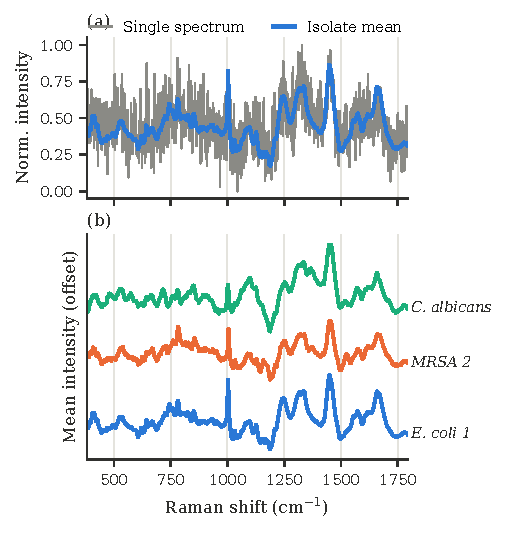
\includegraphics{fig_spectra} finds figures/fig_spectra.pdf
% IEEE asks for subfig (not subfigure/subcaption) with these options:
\usepackage[caption=false,font=footnotesize,labelfont=rm,textfont=rm]{subfig}
\usepackage{tikz}
\usetikzlibrary{positioning,arrows.meta,fit,calc}

% ---------- Algorithms, colour, links ---------------------------------
\usepackage[ruled,linesnumbered]{algorithm2e}
\usepackage{xcolor}
\usepackage[hidelinks]{hyperref}
\usepackage[capitalise,nameinlink]{cleveref}   % load last: \cref{fig:x} -> "Fig. 1"
\crefname{figure}{Fig.}{Figs.}

% ---------- Figure width that suits either layout ---------------------
% In this single-column layout \figwidth is 60% of the page, so plots drawn
% for a 3.5 in journal column are not blown up to full width. If you switch
% to two columns it becomes exactly one column. Use it for normal figures;
% use \textwidth inside figure* for page-wide ones.
\newlength{\figwidth}
\makeatletter
\if@twocolumn\setlength{\figwidth}{\columnwidth}\else\setlength{\figwidth}{0.6\textwidth}\fi
\makeatother

% ---------- Drafting helpers (remove before submission) --------------
\newcommand{\TBD}[1]{\textcolor{red}{[#1]}}
\newcommand{\NOTE}[1]{\textcolor{blue}{\textit{[Note: #1]}}}
% Inserts the image if it exists, otherwise a framed placeholder of the
% same width, so the paper always compiles while figures are pending.
\newcommand{\figorplaceholder}[3][\figwidth]{%
  \IfFileExists{figures/#2}%
    {\includegraphics[width=#1]{#2}}%
    {\fbox{\parbox[c][#3][c]{\dimexpr#1-2\fboxsep-2\fboxrule}{\centering\scriptsize\ttfamily\detokenize{#2}\\(pending)}}}}

% ---------- Symbols used repeatedly -----------------------------------
\newcommand{\wn}{\,cm$^{-1}$}              % 1792.4\wn -> 1792.4 cm^-1
\newcommand{\sunit}[1]{#1\,s}             % \sunit{1}  -> 1 s

\begin{document}

%% =====================================================================
%% 1. TITLE
%% =====================================================================
% Keep the title neutral until results are in. Alternative: "Evaluating 1D
% Residual Networks versus Standard CNNs for Low-SNR Raman Spectroscopy
% Classification". (Text placed between \title and \maketitle ends up on a
% blank first page, so drafting notes for the title live in this comment.)
\title{Do Residual Connections Matter? Evaluating 1D Residual Networks
versus Plain Convolutional Networks for Low-SNR Bacterial Raman Spectroscopy}

\author{Amos~Jaimes,~\TBD{Co-author},~and~\TBD{Senior author}%
\thanks{A. Jaimes is with Northeastern University, Boston, MA, USA
(e-mail: jaimes.a@northeastern.edu).}%
\thanks{\TBD{Funding statement.}}%
\thanks{Manuscript received \TBD{date}.}}

% Running headers are upper-cased by IEEEtran, so no \TBD/\NOTE in here.
\markboth{Journal Name,~Vol.~XX, No.~X, Month~2026}%
{Jaimes \MakeLowercase{\textit{et al.}}: Residual vs.\ Plain 1D CNNs for Raman Spectroscopy}

\maketitle

%% =====================================================================
%% 2. ABSTRACT  (IEEE: one paragraph, 150--250 words, no citations)
%% =====================================================================
\begin{abstract}
\emph{Context.} Rapid, culture-free identification of bacteria from Raman
spectra requires short acquisitions, which produce low signal-to-noise
ratio (SNR) spectra (SNR $\approx 4.1$ at \sunit{1}).
\emph{Objective.} A 25-layer 1D residual network (ResNet) was shown to
outperform classical classifiers on such data, but it is unclear how much
of that gain comes from the residual connections themselves rather than
depth, downsampling strategy or kernel size.
\emph{Methods.} Using the open-access reference dataset of 60{,}000
spectra from 30 bacterial and yeast isolates, we compare a faithful
reimplementation of that ResNet against depth- and width-matched plain
CNNs, and vary one architectural factor at a time: shortcuts, depth
(\TBD{5/10/25} layers), strided convolution versus pooling, and kernel
width.
\emph{Results.} On 30-isolate identification the best plain CNN reaches
\TBD{xx.x\%} and the ResNet \TBD{xx.x\%} (\TBD{$p$}); grouped into eight
empiric-treatment classes, accuracies are \TBD{xx.x\%} and \TBD{xx.x\%}.
For MRSA versus MSSA the ROC-AUC is \TBD{0.xx} versus \TBD{0.xx}.
\TBD{One sentence on noise robustness, gradient flow and convergence.}
\emph{Conclusion.} \TBD{One-sentence architectural recommendation.}
\end{abstract}

\begin{IEEEkeywords}
Raman spectroscopy, deep learning, residual networks, convolutional neural
networks, bacterial identification, antimicrobial resistance, benchmark.
\end{IEEEkeywords}

%% =====================================================================
%% 3. INTRODUCTION
%% =====================================================================
\section{Introduction}
\label{sec:intro}

\IEEEPARstart{R}{apid} identification of pathogenic bacteria is central
to choosing an effective antibiotic early in an infection. Raman
spectroscopy reads a label-free vibrational fingerprint of a cell, but
the acquisition times compatible with high-throughput single-cell
measurement give spectra with very low SNR: about 4.1 for a
\sunit{1} exposure, an order of magnitude below typical reports
\cite{ho2019rapid}.

\paragraph*{Problem statement}
\NOTE{2--3 sentences: why low SNR makes classification hard, and why
deep 1D CNNs are the current answer \cite{liu2017deep,lussier2020deep,pan2021review,zhao2023conincedeep}.}

\paragraph*{Research gap}
Ho~\textit{et al.}~\cite{ho2019rapid} showed that a 25-layer 1D ResNet
\cite{he2016deep} with strided convolutions outperforms logistic
regression and SVMs (82.2\% vs.\ 75.7\% and 74.9\% on 30 isolates).
They report that the ResNet beat simpler MLP and CNN variants, but give
no controlled comparison. It therefore remains unclear how much of the
performance stems from the residual connections themselves versus depth,
kernel choice or the use of strides instead of pooling.

\paragraph*{Contributions}
\begin{enumerate}
  \item A controlled benchmark of plain 1D CNNs against 1D ResNets on the
        open bacteria-ID dataset, matching depth, width and training
        protocol so that the effect of residual connections is isolated.
  \item One-factor-at-a-time ablations of depth, downsampling (strided
        convolution vs.\ max/average pooling) and kernel width.
  \item Evaluation on three clinically motivated tasks (30-isolate
        identification, eight empiric-treatment groups, MRSA vs.\ MSSA)
        and under controlled, simulated SNR degradation.
  \item Training-dynamics, gradient-flow and cost measurements (parameters,
        latency), plus released code and run manifests for every number.
\end{enumerate}

%% =====================================================================
%% 4. DATASET & SPECTRAL REPRESENTATION
%% =====================================================================
\section{Dataset and Spectral Representation}
\label{sec:data}

\subsection{Dataset characteristics}
We use the public bacteria-ID dataset \cite{ho2019rapid}
(\cref{tab:dataset}). The reference set contains 2{,}000 spectra for each
of 30 isolates (60{,}000 total), measured at \sunit{1}. Separate
fine-tuning and test sets, each with 100 spectra per isolate, were
measured at \sunit{2} on independently cultured samples; the longer
exposure compensated for a loss of optical efficiency, so SNR is
comparable across sets. Two clinical sets (2018: 25 patient isolates,
10{,}000 spectra; 2019: 25 isolates, 2{,}500 spectra) cover the five most
common empiric-treatment groups and are labelled by treatment group, not
isolate. \Cref{fig:spectra} shows a single spectrum against its isolate
mean.
\NOTE{Do not claim 1/2/3\,s exposure splits: the release has none.}

% ---- Example: single-column table with booktabs ----------
\begin{table}[!t]
  \centering
  \caption{Splits of the bacteria-ID dataset used in this study.}
  \label{tab:dataset}
  \begin{threeparttable}
  \begin{tabular}{@{}l r c c l@{}}
    \toprule
    Split & {Spectra} & Classes & Exposure & Label space \\
    \midrule
    Reference      & 60000 & 30 & \sunit{1} & isolate \\
    Fine-tune      &  3000 & 30 & \sunit{2} & isolate \\
    Test           &  3000 & 30 & \sunit{2} & isolate \\
    Clinical 2018  & 10000 &  5\tnote{a} & \sunit{1} & treatment \\
    Clinical 2019  &  2500 &  5\tnote{a} & \sunit{2} & treatment \\
    \bottomrule
  \end{tabular}
  \begin{tablenotes}\footnotesize
    \item[a] Treatment groups $\{0,2,3,5,6\}$ of the 8 empiric groups.
  \end{tablenotes}
  \end{threeparttable}
\end{table}

% ---- Example 1: single-column vector figure (PDF from matplotlib) ---
% Generated in the code repo by paper/scripts/make_fig_spectra.py at 3.5 in wide, so it is
% placed at \figwidth (= \columnwidth here) with no scaling and fonts stay
% at 7--8 pt.
\begin{figure}[!t]
  \centering
  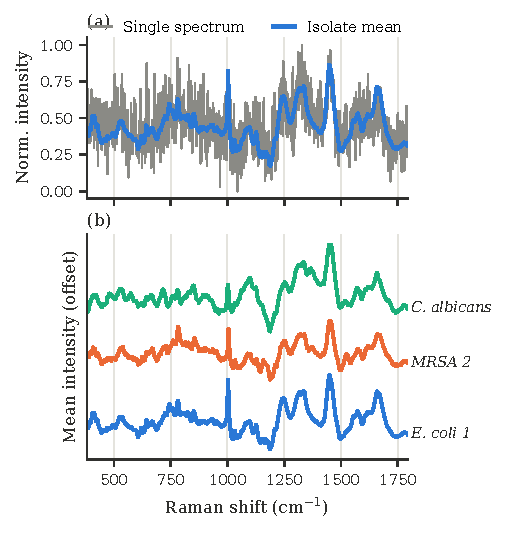
\includegraphics[width=\figwidth]{fig_spectra}
  \caption{(a) One \sunit{1} reference spectrum of \textit{E.~coli}~1
  (grey) against the mean of its 2{,}000 spectra (blue).
  (b) Mean spectra of three isolates, vertically offset.}
  \label{fig:spectra}
\end{figure}

\subsection{Pre-processing and input representation}
Each input is a 1{,}000-point vector over 381.98--1792.4\wn
(1.2\wn steps). The released spectra were already
baseline-corrected with an order-5 polynomial and min--max normalised
to $[0,1]$ by the dataset authors \cite{ho2019rapid}; we apply no further
denoising or baseline steps.
\NOTE{Our ablation found that adding despiking, Savitzky--Golay smoothing
or ASPLS lowers test accuracy (\TBD{74.8\% vs.\ 83.9\%} for the plain
CNN). Report it in \cref{app:preproc}.}

SNR follows the definition of \cite{ho2019rapid}:
\begin{equation}
  \mathrm{SNR} = \frac{\max_k x_k - \min_k x_k}
                      {\max_{k\in\mathcal{W}} x_k - \min_{k\in\mathcal{W}} x_k},
  \label{eq:snr}
\end{equation}
where $\mathcal{W}$ is a 20-pixel window with no Raman signal.

\subsection{Evaluation protocol}
Following \cite{ho2019rapid}, every model is pre-trained on the reference
set and then fine-tuned on the fine-tuning set. We repeat fine-tuning
over five random 90/10 train/validation splits, select checkpoints on
validation accuracy only, and evaluate once on the independently cultured
test set. Each configuration is run with \TBD{3--5} seeds. The released
data carry no sample or batch IDs, so sample-level cross-validation within
the reference set is not possible; the separately prepared test set
provides that guarantee instead.

%% =====================================================================
%% 5. MODEL ARCHITECTURES & EXPERIMENTAL SETUP
%% =====================================================================
\section{Model Architectures and Experimental Setup}
\label{sec:models}

We compare two families of convolutional neural networks (CNNs)
\cite{lecun1998gradient} of the kind used for 1D vibrational and Raman
spectra \cite{acquarelli2017convolutional,liu2017deep,deng2022scale}: a 1D
residual network (ResNet) \cite{he2016deep} and a plain CNN without
shortcut connections \cite{lecun1998gradient}. Both networks map one
spectrum of $1{\times}1000$ points, min--max normalised to $[0,1]$ with
RamanSPy~0.2.10 \cite{georgiev2024ramanspy}, to 30 isolate logits, and both
are implemented in PyTorch \cite{paszke2019pytorch}. \Cref{fig:arch} draws
the two networks layer by layer, \cref{fig:blocks} compares their building
blocks, and \cref{tab:configs} lists their attributes next to the ResNet-25
of Ho~\textit{et al.}\ \cite{ho2019rapid,ho2019bacteriaid}, which serves as a
reference and was not trained here.

\subsection{1D ResNet}
\label{sec:models-resnet}
The 1D ResNet transfers the stage layout of ResNet-18, four stages of two
basic blocks each, to one spatial dimension, with every stage width reduced
four-fold (16--128 channels instead of 64--512) \cite{he2016deep}. A stem
convolution (16 filters, kernel 7, stride 2) followed by batch
normalisation (BN) \cite{ioffe2015batch}, a rectified linear unit (ReLU)
\cite{nair2010rectified} and max pooling (kernel 3, stride 2) reduces the
input to $16{\times}250$, as the stem of \cite{he2016deep} does for images.
Each basic block (\cref{fig:blocks}(a)) computes
\begin{equation}
  \mathbf{y} = \sigma\!\bigl(\mathrm{BN}(\mathbf{W}_2 * \sigma(\mathrm{BN}(\mathbf{W}_1 *_s \mathbf{x})))
               + \mathcal{S}(\mathbf{x})\bigr),
  \label{eq:block}
\end{equation}
where $*_s$ is a kernel-3 convolution with stride $s$, $\sigma$ is the ReLU
and $\mathcal{S}$ is the shortcut; this is the original post-activation
ordering of \cite{he2016deep}, not the pre-activation variant of
\cite{he2016identity}. The shortcut is the identity when a block keeps its
length and width, and otherwise a $1{\times}1$ convolution with stride $s$
followed by BN, i.e.\ the projection shortcut of \cite{he2016deep}. The
four stages have 16, 32, 64 and 128 channels, and the first block of
stages 2--4 has stride 2, so the feature length falls from 250 to 125, 63
and 32 \cite{he2016deep}. Global average pooling (GAP) \cite{lin2014network}
reduces the $128{\times}32$ map to 128 features, which pass through a
128-unit linear layer, a ReLU \cite{nair2010rectified}, dropout with
$p=0.4$ \cite{srivastava2014dropout} and a 30-way linear classifier.

The network has 17 convolutions on its main path plus 3 projection
convolutions; each of the 20 convolutions is followed by BN and therefore
has no bias, since the BN shift subsumes it \cite{ioffe2015batch}. It has
262{,}510 trainable parameters, and the theoretical receptive field of its
last main-path convolution covers 435 of the 1{,}000 input points, an upper
bound on the region that effectively influences a unit
\cite{luo2016understanding}.

\subsection{Plain 1D CNN}
\label{sec:models-cnn}
The plain CNN is a PyTorch \cite{paszke2019pytorch} port of the six-layer
Keras CNN used in our group's earlier work, a conventional stack of
convolution and pooling layers \cite{lecun1998gradient} of the type applied
to spectra in \cite{acquarelli2017convolutional,liu2017deep}. Each of its
six blocks (\cref{fig:blocks}(b)) applies a kernel-3 convolution with
bias, a ReLU \cite{nair2010rectified} and BN, so normalisation follows the
non-linearity instead of preceding it as proposed in \cite{ioffe2015batch}.
Blocks 1--5 end with average pooling (kernel 3, stride 3), which shortens
the feature map from 1{,}000 to 333, 111, 37, 12 and 4 points
\cite{lecun1998gradient}, and block 6 feeds GAP \cite{lin2014network}
directly. The blocks have 8, 16, 32, 32, 64 and 128 channels, and the
128 pooled features pass through dropout with $p=0.3$
\cite{srivastava2014dropout} to a single 30-way linear layer
\cite{lin2014network}. The network has no shortcuts, no strided
convolutions and no hidden fully connected layer; it contains 6
convolutions, each followed by BN \cite{ioffe2015batch}, and 40{,}446
trainable parameters.
Because every pooling step triples the sampling interval, its theoretical
receptive field reaches 971 points, nearly the whole spectrum
\cite{luo2016understanding}.

% ---- Fig. A: both networks, layer by layer ---------------------------
\begin{figure*}[!t]
  \centering
  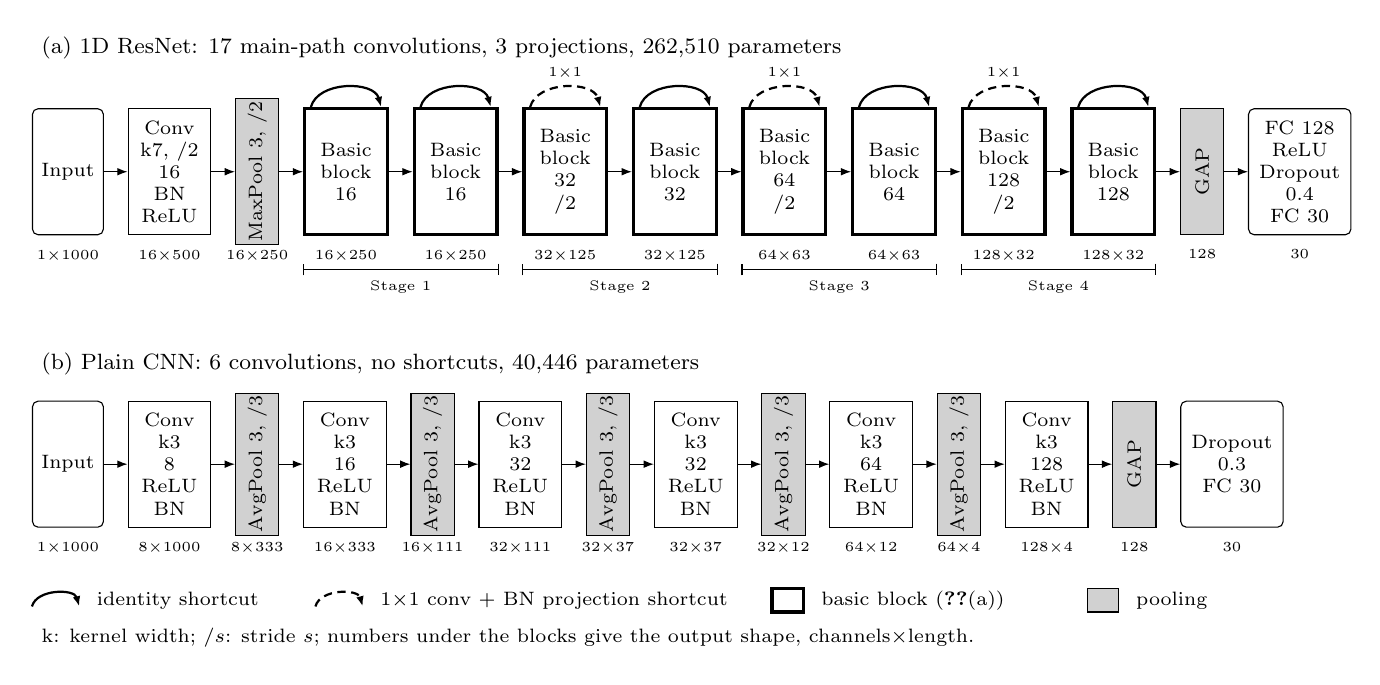
\begin{tikzpicture}[
      font=\scriptsize,
      node distance=3mm,
      box/.style={draw, minimum height=16mm, align=center, inner sep=1pt},
      io/.style={box, rounded corners=2pt, minimum width=9mm},
      cv/.style={box, minimum width=10.5mm},
      rb/.style={box, very thick, minimum width=10.5mm},
      pl/.style={box, fill=black!18, minimum width=5.5mm},
      hd/.style={box, rounded corners=2pt, minimum width=13mm},
      shp/.style={font=\tiny, below=0.6mm},
      arr/.style={-{Latex[length=1.3mm]}},
      sc/.style={-{Latex[length=1.3mm]}, thick},
      pj/.style={sc, densely dashed},
      stg/.style={{|[width=1.5mm]}-{|[width=1.5mm]}, thin}]
    % ---------------- (a) 1D ResNet ----------------
    \node[io] (a0) {Input};
    \node[cv, right=of a0] (a1) {Conv\\k7, /2\\16\\BN\\ReLU};
    \node[pl, right=of a1] (a2) {\rotatebox{90}{MaxPool 3, /2}};
    \node[rb, right=of a2] (b1) {Basic\\block\\16};
    \node[rb, right=of b1] (b2) {Basic\\block\\16};
    \node[rb, right=of b2] (b3) {Basic\\block\\32\\/2};
    \node[rb, right=of b3] (b4) {Basic\\block\\32};
    \node[rb, right=of b4] (b5) {Basic\\block\\64\\/2};
    \node[rb, right=of b5] (b6) {Basic\\block\\64};
    \node[rb, right=of b6] (b7) {Basic\\block\\128\\/2};
    \node[rb, right=of b7] (b8) {Basic\\block\\128};
    \node[pl, right=of b8] (a3) {\rotatebox{90}{GAP}};
    \node[hd, right=of a3] (a4) {FC 128\\ReLU\\Dropout\\0.4\\FC 30};
    \foreach \u/\v in {a0/a1,a1/a2,a2/b1,b1/b2,b2/b3,b3/b4,b4/b5,b5/b6,
                       b6/b7,b7/b8,b8/a3,a3/a4}
      \draw[arr] (\u) -- (\v);
    \foreach \n/\s in {a0/1{\times}1000,a1/16{\times}500,a2/16{\times}250,
                       b1/16{\times}250,b2/16{\times}250,b3/32{\times}125,
                       b4/32{\times}125,b5/64{\times}63,b6/64{\times}63,
                       b7/128{\times}32,b8/128{\times}32,a3/128,a4/30}
      \node[shp] at (\n.south |- a0.south) {$\s$};
    % shortcuts: solid = identity, dashed = 1x1 conv + BN projection
    \foreach \n in {b1,b2,b4,b6,b8}
      \draw[sc] ($(\n.north west)+(1mm,0)$) to[bend left=75] ($(\n.north east)+(-1mm,0)$);
    \foreach \n in {b3,b5,b7}
      \draw[pj] ($(\n.north west)+(1mm,0)$) to[bend left=75]
            node[above=-0.3mm, font=\tiny] {$1{\times}1$} ($(\n.north east)+(-1mm,0)$);
    % stage brackets
    \foreach \p/\q/\t in {b1/b2/Stage 1,b3/b4/Stage 2,b5/b6/Stage 3,b7/b8/Stage 4}
      \draw[stg] ($(\p.south west)+(0,-4.2mm)$) -- node[below=0.3mm, font=\tiny] {\t}
                 ($(\q.south east)+(0,-4.2mm)$);
    \node[anchor=south west, font=\footnotesize] at ($(a0.north west)+(0,5mm)$)
         {(a) 1D ResNet: 17 main-path convolutions, 3 projections, 262{,}510 parameters};
    % ---------------- (b) plain CNN ----------------
    \node[io, below=21mm of a0] (c0) {Input};
    \node[cv, right=of c0] (c1) {Conv\\k3\\8\\ReLU\\BN};
    \node[pl, right=of c1] (p1) {\rotatebox{90}{AvgPool 3, /3}};
    \node[cv, right=of p1] (c2) {Conv\\k3\\16\\ReLU\\BN};
    \node[pl, right=of c2] (p2) {\rotatebox{90}{AvgPool 3, /3}};
    \node[cv, right=of p2] (c3) {Conv\\k3\\32\\ReLU\\BN};
    \node[pl, right=of c3] (p3) {\rotatebox{90}{AvgPool 3, /3}};
    \node[cv, right=of p3] (c4) {Conv\\k3\\32\\ReLU\\BN};
    \node[pl, right=of c4] (p4) {\rotatebox{90}{AvgPool 3, /3}};
    \node[cv, right=of p4] (c5) {Conv\\k3\\64\\ReLU\\BN};
    \node[pl, right=of c5] (p5) {\rotatebox{90}{AvgPool 3, /3}};
    \node[cv, right=of p5] (c6) {Conv\\k3\\128\\ReLU\\BN};
    \node[pl, right=of c6] (g)  {\rotatebox{90}{GAP}};
    \node[hd, right=of g]  (h)  {Dropout\\0.3\\FC 30};
    \foreach \u/\v in {c0/c1,c1/p1,p1/c2,c2/p2,p2/c3,c3/p3,p3/c4,c4/p4,
                       p4/c5,c5/p5,p5/c6,c6/g,g/h}
      \draw[arr] (\u) -- (\v);
    \foreach \n/\s in {c0/1{\times}1000,c1/8{\times}1000,p1/8{\times}333,
                       c2/16{\times}333,p2/16{\times}111,c3/32{\times}111,
                       p3/32{\times}37,c4/32{\times}37,p4/32{\times}12,
                       c5/64{\times}12,p5/64{\times}4,c6/128{\times}4,g/128,h/30}
      \node[shp] at (\n.south |- c0.south) {$\s$};
    \node[anchor=south west, font=\footnotesize] at ($(c0.north west)+(0,2mm)$)
         {(b) Plain CNN: 6 convolutions, no shortcuts, 40{,}446 parameters};
    % ---------------- legend ----------------
    \begin{scope}[shift={($(c0.south west)+(0,-10mm)$)}, font=\scriptsize]
      \draw[sc] (0,0) to[bend left=75] (6mm,0);
      \node[anchor=west] at (7mm,0.8mm) {identity shortcut};
      \draw[pj] (36mm,0) to[bend left=75] (42mm,0);
      \node[anchor=west] at (43mm,0.8mm) {$1{\times}1$ conv + BN projection shortcut};
      \node[draw, very thick, minimum width=4mm, minimum height=3mm] at (96mm,0.8mm) {};
      \node[anchor=west] at (99mm,0.8mm) {basic block (\cref{fig:blocks}(a))};
      \node[draw, fill=black!18, minimum width=4mm, minimum height=3mm] at (136mm,0.8mm) {};
      \node[anchor=west] at (139mm,0.8mm) {pooling};
      \node[anchor=west] at (0,-4mm) {k: kernel width; /$s$: stride $s$;
        numbers under the blocks give the output shape, channels${\times}$length.};
    \end{scope}
  \end{tikzpicture}
  \caption{The two networks compared in this study, drawn layer by layer
  with the output shape of every layer. (a) 1D ResNet: a strided stem and
  max pooling, then four stages of two basic blocks whose shortcuts are
  identities (solid arcs) or $1{\times}1$ projections where the stride or
  width changes (dashed arcs). (b) Plain CNN: six convolution blocks, the
  first five followed by average pooling (grey) and the last by global
  average pooling.}
  \label{fig:arch}
\end{figure*}

% ---- Fig. B: building blocks -----------------------------------------
\begin{figure}[!t]
  \centering
  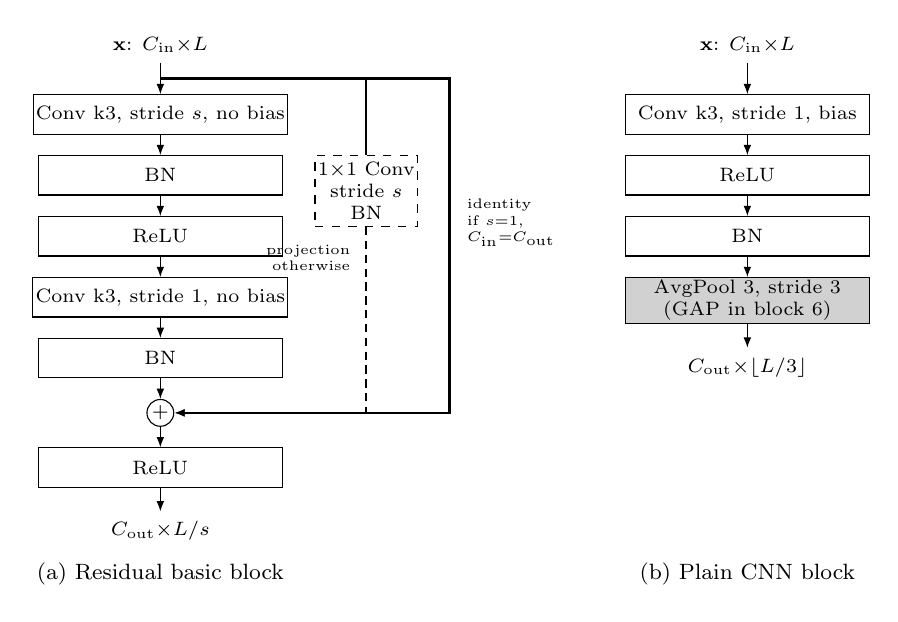
\begin{tikzpicture}[
      font=\scriptsize,
      node distance=2.6mm,
      op/.style={draw, minimum width=31mm, minimum height=5mm, align=center, inner sep=1pt},
      pl/.style={op, fill=black!18},
      arr/.style={-{Latex[length=1.3mm]}},
      sc/.style={-{Latex[length=1.3mm]}, thick}]
    % ---------------- (a) residual basic block ----------------
    \node (xin) {$\mathbf{x}$: $C_\mathrm{in}{\times}L$};
    \node[op, below=4mm of xin] (r1) {Conv k3, stride $s$, no bias};
    \node[op, below=of r1] (r2) {BN};
    \node[op, below=of r2] (r3) {ReLU};
    \node[op, below=of r3] (r4) {Conv k3, stride 1, no bias};
    \node[op, below=of r4] (r5) {BN};
    \node[draw, circle, inner sep=0.6pt, below=of r5] (add) {$+$};
    \node[op, below=of add] (r6) {ReLU};
    \node[below=3mm of r6] (yout) {$C_\mathrm{out}{\times}L/s$};
    \draw[arr] (xin) -- (r1);
    \foreach \u/\v in {r1/r2,r2/r3,r3/r4,r4/r5,r5/add,add/r6,r6/yout}
      \draw[arr] (\u) -- (\v);
    % shortcut: fork into identity lane and projection lane, rejoin at +
    \coordinate (fork) at ($(xin.south)!0.5!(r1.north)$);
    \node[op, dashed, minimum width=13mm, minimum height=9mm, anchor=north west]
         (proj) at ($(r2.north east)+(4mm,0)$) {$1{\times}1$ Conv\\stride $s$\\BN};
    \coordinate (laneI) at ($(proj.east)+(4mm,0)$);
    \draw[thick] (fork) -| (proj.north);
    \draw[thick, densely dashed, arr] (proj.south) |- (add.east);
    \draw[sc] (fork) -| (laneI |- add) -- (add.east);
    \node[font=\tiny, align=left, anchor=west] at ($(laneI)+(1mm,-4mm)$) {identity\\if $s{=}1$,\\$C_\mathrm{in}{=}C_\mathrm{out}$};
    \node[font=\tiny, align=right, anchor=north east] at ($(proj.south)+(-0.8mm,-1mm)$) {projection\\otherwise};
    \coordinate (cap) at ($(yout.south)+(0,-3mm)$);
    \node[font=\footnotesize] at (cap) {(a) Residual basic block};
    % ---------------- (b) plain CNN block ----------------
    \node[right=60mm of xin] (pin) {$\mathbf{x}$: $C_\mathrm{in}{\times}L$};
    \node[op, below=4mm of pin] (q1) {Conv k3, stride 1, bias};
    \node[op, below=of q1] (q2) {ReLU};
    \node[op, below=of q2] (q3) {BN};
    \node[pl, below=of q3] (q4) {AvgPool 3, stride 3\\(GAP in block 6)};
    \node[below=3mm of q4] (pout) {$C_\mathrm{out}{\times}\lfloor L/3\rfloor$};
    \draw[arr] (pin) -- (q1);
    \foreach \u/\v in {q1/q2,q2/q3,q3/q4,q4/pout}
      \draw[arr] (\u) -- (\v);
    \node[font=\footnotesize] at (pout |- cap) {(b) Plain CNN block};
  \end{tikzpicture}
  \caption{Building blocks. (a) Residual basic block of the 1D ResNet, with
  BN before each ReLU and the shortcut added before the last ReLU; the
  shortcut is the identity (solid) unless the block changes stride or
  width, in which case a $1{\times}1$ convolution with BN projects it
  (dashed). (b) Block of the plain CNN, with BN after the ReLU and average
  pooling (grey) instead of a strided convolution.}
  \label{fig:blocks}
\end{figure}

\subsection{Scope of the comparison}
\label{sec:models-scope}
The two networks differ in several factors at once
(\cref{fig:arch,tab:configs}), so the comparison is between two architecture
families trained under one identical protocol, not a single-factor ablation
of residual connections \cite{he2016deep}. The factors are:
\begin{enumerate}
  \item \emph{Shortcuts.} Residual connections ease the optimisation of
        deep stacks \cite{he2016deep,he2016identity}, whose gradients can
        otherwise vanish or explode \cite{bengio1994learning,glorot2010understanding}.
  \item \emph{Depth.} The ResNet has 17 main-path convolutions and the plain
        CNN 6, and depth alone changes how hard a network is to train
        \cite{glorot2010understanding,he2016deep}.
  \item \emph{Receptive field.} Both use kernel-3 body convolutions, but
        the plain CNN's three-fold pooling gives it a 971-point theoretical
        receptive field against 435 for the ResNet; the effective
        receptive field is smaller than the theoretical one in both cases
        \cite{luo2016understanding}.
  \item \emph{Downsampling.} The ResNet downsamples with strided
        convolutions and one max-pooling layer, the plain CNN with fixed
        average pooling; learned strided convolution and pooling are not
        interchangeable \cite{springenberg2015striving}.
  \item \emph{Normalisation placement.} BN precedes the ReLU in the ResNet,
        as in \cite{ioffe2015batch,he2016deep}, and follows it in the plain
        CNN \cite{ioffe2015batch}.
  \item \emph{Head and regularisation.} The ResNet adds a 128-unit hidden
        layer with dropout 0.4, the plain CNN a linear classifier after
        dropout 0.3 \cite{srivastava2014dropout,lin2014network}.
  \item \emph{Capacity.} The ResNet has 6.5 times as many parameters
        (262{,}510 vs.\ 40{,}446), whereas the plain and residual networks
        of \cite{he2016deep} were matched in depth, width and parameter count.
\end{enumerate}
A difference between the two families can therefore not be attributed to
the shortcuts alone \cite{he2016deep}. Neither network is the ResNet-25 of
\cite{ho2019rapid}, which uses 100 channels, kernel-5 convolutions, no
pooling and a flattened $100{\times}32$ head, has 1{,}340{,}878 parameters
and was trained with Adam ($\beta=(0.5,0.999)$) at batch size 10
\cite{ho2019bacteriaid}; \cref{tab:configs} lists it only as a reference.

\begin{table}[!t]
  \centering
  \caption{Architectures compared. Shapes are channels${\times}$length;
  ``/2'' denotes stride 2. The ResNet-25 column is a reference taken from
  the released code of \cite{ho2019rapid} and was not trained here.}
  \label{tab:configs}
  \begin{threeparttable}
  \begin{tabular}{@{}l p{4.7cm} p{4.4cm} p{4.4cm}@{}}
    \toprule
    Attribute & 1D ResNet (ours) & Plain CNN (ours) & ResNet-25 \cite{ho2019rapid,ho2019bacteriaid}\tnote{a} \\
    \midrule
    Stem & Conv k7, /2, 16 ch; BN; ReLU; MaxPool 3, /2 & none & Conv k5, 64 ch; BN; ReLU \\
    Body & 4 stages ${\times}$ 2 basic blocks & 6 conv blocks & 6 stages ${\times}$ 2 basic blocks \\
    Channels & 16, 32, 64, 128 & 8, 16, 32, 32, 64, 128 & 100 in every stage \\
    Body kernel width & 3 & 3 & 5 \\
    Main-path convolutions & 17 & 6 & 25 \\
    Shortcuts & 5 identity, 3 projection & none & 6 identity, 6 projection \\
    BN placement & after each conv, before ReLU & after ReLU & after each conv, before ReLU \\
    Downsampling & strided stem, max pool, stride 2 in stages 2--4 & average pool 3, /3 after blocks 1--5 & stride 2 in stages 2--6, no pooling \\
    Map before head & $128{\times}32$ & $128{\times}4$ & $100{\times}32$ \\
    Head & GAP; FC 128; ReLU; dropout 0.4; FC 30 & GAP; dropout 0.3; FC 30 & flatten (3{,}200); FC 30 \\
    Receptive field (points) & 435 & 971 & 889 \\
    Trainable parameters & 262{,}510 & 40{,}446 & 1{,}340{,}878 \\
    Trained in this study & yes & yes & no \\
    \bottomrule
  \end{tabular}
  \begin{tablenotes}\footnotesize
    \item[a] Not trained here; attributes read from \texttt{resnet.py} and
    \texttt{1\_reference\_finetuning.ipynb} of \cite{ho2019bacteriaid}.
  \end{tablenotes}
  \end{threeparttable}
\end{table}

\subsection{Training protocol}
\label{sec:models-training}
Both networks are trained with the same protocol (\cref{fig:pipeline,tab:hparams}),
which follows the pre-train and fine-tune scheme of \cite{ho2019rapid} but
not its hyper-parameters \cite{ho2019bacteriaid}. All stages minimise the
cross-entropy
$\mathcal{L} = -\frac{1}{N}\sum_{i}\log p_\theta(y_i\mid\mathbf{x}_i)$
without label smoothing \cite{szegedy2016rethinking} and without class
weights, since every isolate contributes 2{,}000 reference spectra
\cite{ho2019rapid}.

\emph{Pre-training.} The 60{,}000 reference spectra \cite{ho2019rapid} are
split at random (seeded, not stratified) into 67\% for training (40{,}200)
and 33\% for validation (19{,}800), and the validation part is used only
for early stopping \cite{prechelt1998early}. We use Adam
\cite{kingma2015adam} with learning rate $10^{-3}$, the default
$\beta=(0.9,0.999)$ and batch size 64. A weight decay of 0.01 is applied as
the coupled L2 penalty of \texttt{torch.optim.Adam}
\cite{paszke2019pytorch}, which under adaptive learning rates is not
equivalent to the decoupled weight decay of AdamW
\cite{loshchilov2019decoupled}. The learning rate follows a cosine
annealing schedule without restarts \cite{loshchilov2017sgdr}, with
$T_{\max}=100$ epochs and one step per epoch. Training runs for at most 100
epochs and stops when the validation loss has not improved for 10 epochs,
after which the weights with the lowest validation loss are restored
\cite{prechelt1998early}. According to the run manifests released with the
code, the ResNet stopped after 40, 100 and 100 epochs and the plain CNN
after 56, 100 and 100 epochs for seeds 1, 2 and 3. Training spectra, and only those, are augmented
on the fly by a circular shift of an integer number of points in
$[-5,5]$, additive Gaussian noise with $\sigma=0.01$ and a multiplicative
scale drawn from $\mathcal{U}(0.95,1.05)$, in the spirit of the shift and
noise augmentation of \cite{liu2017deep}; mixup \cite{zhang2018mixup} is
not used.

\emph{Fine-tuning.} The pre-trained network is then fine-tuned on the
3{,}000-spectrum fine-tuning set (100 spectra per isolate at \sunit{2})
\cite{ho2019rapid}, with all layers updated. Fine-tuning uses Adam
\cite{kingma2015adam} at learning rate $10^{-4}$ (one tenth of the
pre-training rate), no weight decay, batch size 64 and a cosine schedule
with $T_{\max}=20$ \cite{loshchilov2017sgdr} for 20 epochs, without
augmentation. The fine-tuning set is not split, so no early stopping is
possible and the weights after the last epoch are kept
\cite{prechelt1998early}.

\emph{Testing.} Each fine-tuned network is evaluated in a single pass over
the 3{,}000 spectra of the independently cultured test set
\cite{ho2019rapid}; no checkpoint, hyper-parameter or threshold is
selected on it \cite{dietterich1998approximate}.

\emph{Seeds, hardware and software.} Each network is trained with seeds 1,
2 and 3, which seed the Python, NumPy \cite{harris2020array} and PyTorch
\cite{paszke2019pytorch} generators, the reference split and the data
loaders; cuDNN runs in deterministic mode with benchmarking disabled
\cite{paszke2019pytorch}. All reported runs used one GPU
(\cref{sec:models-hardware}) with Python~3.12.10,
PyTorch~2.11.0+cu128 \cite{paszke2019pytorch},
NumPy~2.5.2 \cite{harris2020array} and RamanSPy~0.2.10
\cite{georgiev2024ramanspy}. The run manifests record that one run
(pre-training, fine-tuning and test) took 9.7, 25.8 and 23.3\,min for the
ResNet and 8.2, 14.5 and 14.6\,min for the plain CNN (seeds 1--3) on this
GPU.

% ---- Fig. C: experimental pipeline -----------------------------------
\begin{figure}[!t]
  \centering
  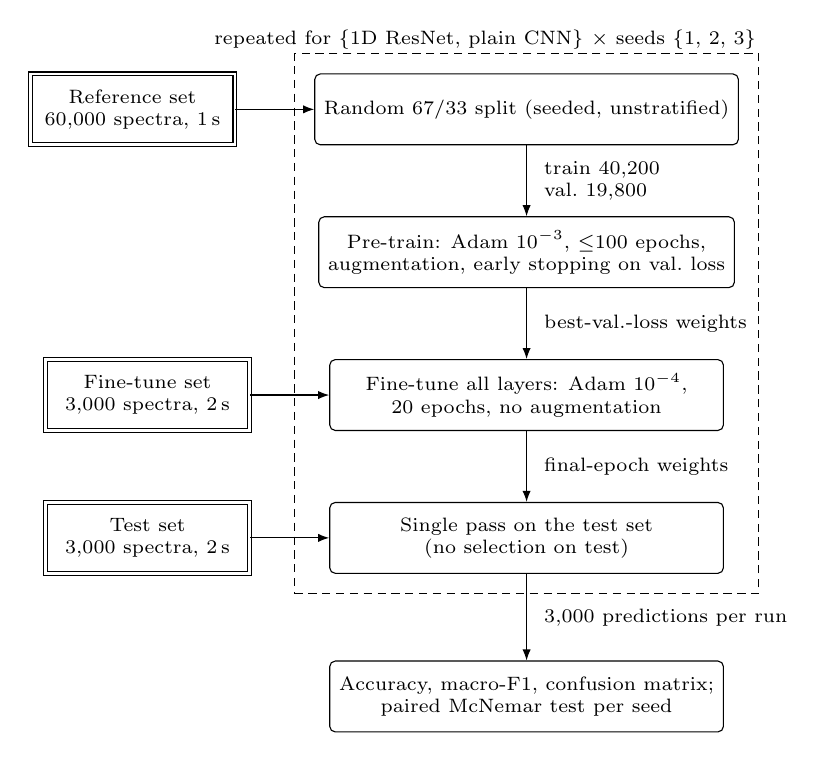
\begin{tikzpicture}[
      font=\scriptsize,
      node distance=5mm,
      data/.style={draw, double, double distance=1pt, minimum width=26mm,
                   minimum height=9mm, align=center},
      proc/.style={draw, rounded corners=2pt, minimum width=50mm,
                   minimum height=9mm, align=center},
      arr/.style={-{Latex[length=1.4mm]}},
      lab/.style={font=\scriptsize, align=left}]
    \node[proc] (split) {Random 67/33 split (seeded, unstratified)};
    \node[proc, below=9mm of split] (pre) {Pre-train: Adam $10^{-3}$, $\le$100 epochs,\\
          augmentation, early stopping on val.\ loss};
    \node[proc, below=9mm of pre] (ft) {Fine-tune all layers: Adam $10^{-4}$,\\
          20 epochs, no augmentation};
    \node[proc, below=9mm of ft] (test) {Single pass on the test set\\(no selection on test)};
    \node[proc, below=11mm of test] (stats) {Accuracy, macro-F1, confusion matrix;\\
          paired McNemar test per seed};
    \node[data, left=10mm of split] (ref) {Reference set\\60{,}000 spectra, \sunit{1}};
    \node[data, left=10mm of ft]    (fts) {Fine-tune set\\3{,}000 spectra, \sunit{2}};
    \node[data, left=10mm of test]  (tst) {Test set\\3{,}000 spectra, \sunit{2}};
    \draw[arr] (ref) -- (split);
    \draw[arr] (fts) -- (ft);
    \draw[arr] (tst) -- (test);
    \draw[arr] (split) -- node[lab, right=1mm] {train 40{,}200\\val.\ 19{,}800} (pre);
    \draw[arr] (pre) -- node[lab, right=1mm] {best-val.-loss weights} (ft);
    \draw[arr] (ft) -- node[lab, right=1mm] {final-epoch weights} (test);
    \draw[arr] (test) -- node[lab, right=1mm] {3{,}000 predictions per run} (stats);
    \node[draw, densely dashed, inner sep=2.5mm, fit=(split)(pre)(ft)(test)] (rep) {};
    \node[font=\scriptsize, anchor=south east, inner sep=1pt] at (rep.north east)
         {repeated for \{1D ResNet, plain CNN\} ${\times}$ seeds \{1, 2, 3\}};
  \end{tikzpicture}
  \caption{Experimental pipeline. Everything inside the dashed box is run
  identically for both networks and for each of the three seeds; double
  borders mark data sets. The test set is touched once per run, and the
  paired statistics compare the two networks seed by seed.}
  \label{fig:pipeline}
\end{figure}

\begin{table}[!t]
  \centering
  \caption{Training protocol shared by both networks. It differs from that
  of \cite{ho2019bacteriaid} (Adam with $\beta=(0.5,0.999)$, batch size 10).}
  \label{tab:hparams}
  \begin{tabular}{@{}l p{6.6cm} p{5.0cm}@{}}
    \toprule
    Setting & Pre-training & Fine-tuning \\
    \midrule
    Data & reference set, random 67/33 split: 40{,}200 train, 19{,}800 val. & fine-tune set, all 3{,}000 spectra \\
    Layers updated & all & all \\
    Loss & cross-entropy, no label smoothing, no class weights & same \\
    Optimiser & Adam, $\beta=(0.9,0.999)$ & Adam, $\beta=(0.9,0.999)$ \\
    Learning rate & $10^{-3}$ & $10^{-4}$ \\
    Weight decay & 0.01, coupled L2 (\texttt{torch.optim.Adam}) & none \\
    Batch size & 64 & 64 \\
    Schedule & cosine, $T_{\max}=100$ epochs, stepped per epoch & cosine, $T_{\max}=20$ epochs \\
    Epochs & at most 100 & 20 \\
    Early stopping & val.\ loss, patience 10, best weights restored & none, final-epoch weights \\
    Augmentation & circular shift in $[-5,5]$ points; Gaussian noise $\sigma=0.01$; scale $\mathcal{U}(0.95,1.05)$ & none \\
    \midrule
    Seeds & \multicolumn{2}{l}{1, 2, 3 (Python, NumPy, PyTorch, split, loaders); cuDNN deterministic, benchmark off} \\
    Hardware & \multicolumn{2}{l}{one GPU (\cref{sec:models-hardware})} \\
    \bottomrule
  \end{tabular}
\end{table}

\subsection{Evaluation metrics and statistical analysis}
\label{sec:models-stats}
From the test predictions we compute accuracy, macro-F1 (the unweighted
mean of the 30 per-class F1 scores), per-class precision and recall, and the
confusion matrix with NumPy \cite{harris2020array}. For each seed, the two
networks are compared with McNemar's test on per-spectrum correctness over
the same 3{,}000 test spectra \cite{mcnemar1947note,dietterich1998approximate},
using Edwards' continuity correction \cite{edwards1948note}:
\begin{equation}
  \chi^2 = \frac{(\lvert b-c\rvert-1)^2}{b+c},
  \label{eq:mcnemar}
\end{equation}
where $b$ and $c$ count the spectra that only one of the two networks
classifies correctly, and $\chi^2$ is referred to a $\chi^2$ distribution
with one degree of freedom \cite{mcnemar1947note}. McNemar's test captures
the sampling variation of the test set but not the variation due to
training \cite{dietterich1998approximate}, so we also report mean $\pm$
standard deviation over the three seeds and a paired $t$-interval on the
per-seed differences, which with three seeds has only two degrees of
freedom \cite{dietterich1998approximate}.

\subsection{Computing hardware}
\label{sec:models-hardware}
The experiments used two machines: a workstation with an NVIDIA GeForce
RTX~3060 GPU, driven through PyTorch's CUDA backend
\cite{paszke2019pytorch}, and an Apple Mac with an M3 chip, driven through
PyTorch's Metal Performance Shaders (MPS) backend \cite{pytorchmps}. All
runs whose numbers we report (both networks, seeds 1--3) ran on the
RTX~3060, as their run manifests record. The Mac M3 was used for earlier
development runs, whose logs record the MPS device.

\NOTE{Plain-N depth, downsampling and kernel ablations listed in the
abstract/introduction are not yet implemented; either run them or remove
them from the abstract and contributions.}

%% =====================================================================
%% 6. RESULTS
%% =====================================================================
\section{Results}
\label{sec:results}

\subsection{30-isolate species classification}
\label{sec:res-isolate}
\Cref{tab:main} summarises test accuracy and macro-F1.
\NOTE{Lead with the controlled ResNet-25 vs.\ Plain-25 contrast, then depth.}

% ---- Main results table with mean $\pm$ s.d. ------------------
\begin{table}[!t]
  \centering
  \caption{Test-set performance. Our rows give mean $\pm$ s.d.\ over
  three seeds, one test pass each. n.e.: not evaluated.
  $^\dagger$As reported in \cite{ho2019rapid}.}
  \label{tab:main}
  \begin{tabular}{@{}l c c c@{}}
    \toprule
    Model & 30-isolate (\%) & Treatment (\%) & MRSA AUC \\
    \midrule
    LR \cite{ho2019rapid}       & 75.7 & 93.3 & -- \\
    SVM \cite{ho2019rapid}      & 74.9 & 92.2 & -- \\
    ResNet-25$^\dagger$ \cite{ho2019rapid} & 82.2\,$\pm$\,0.3 & 97.0\,$\pm$\,0.3 & 0.953 \\
    \midrule
    1D ResNet (ours)            & 79.6\,$\pm$\,1.8 & n.e. & n.e. \\
    Plain CNN (ours)            & 83.9\,$\pm$\,0.3 & n.e. & n.e. \\
    \bottomrule
  \end{tabular}
\end{table}

% ---- Example 3: full-width figure with two sub-figures (figure*) ---
\begin{figure*}[!t]
  \centering
  \subfloat[Plain CNN\label{fig:cm-plain}]{%
    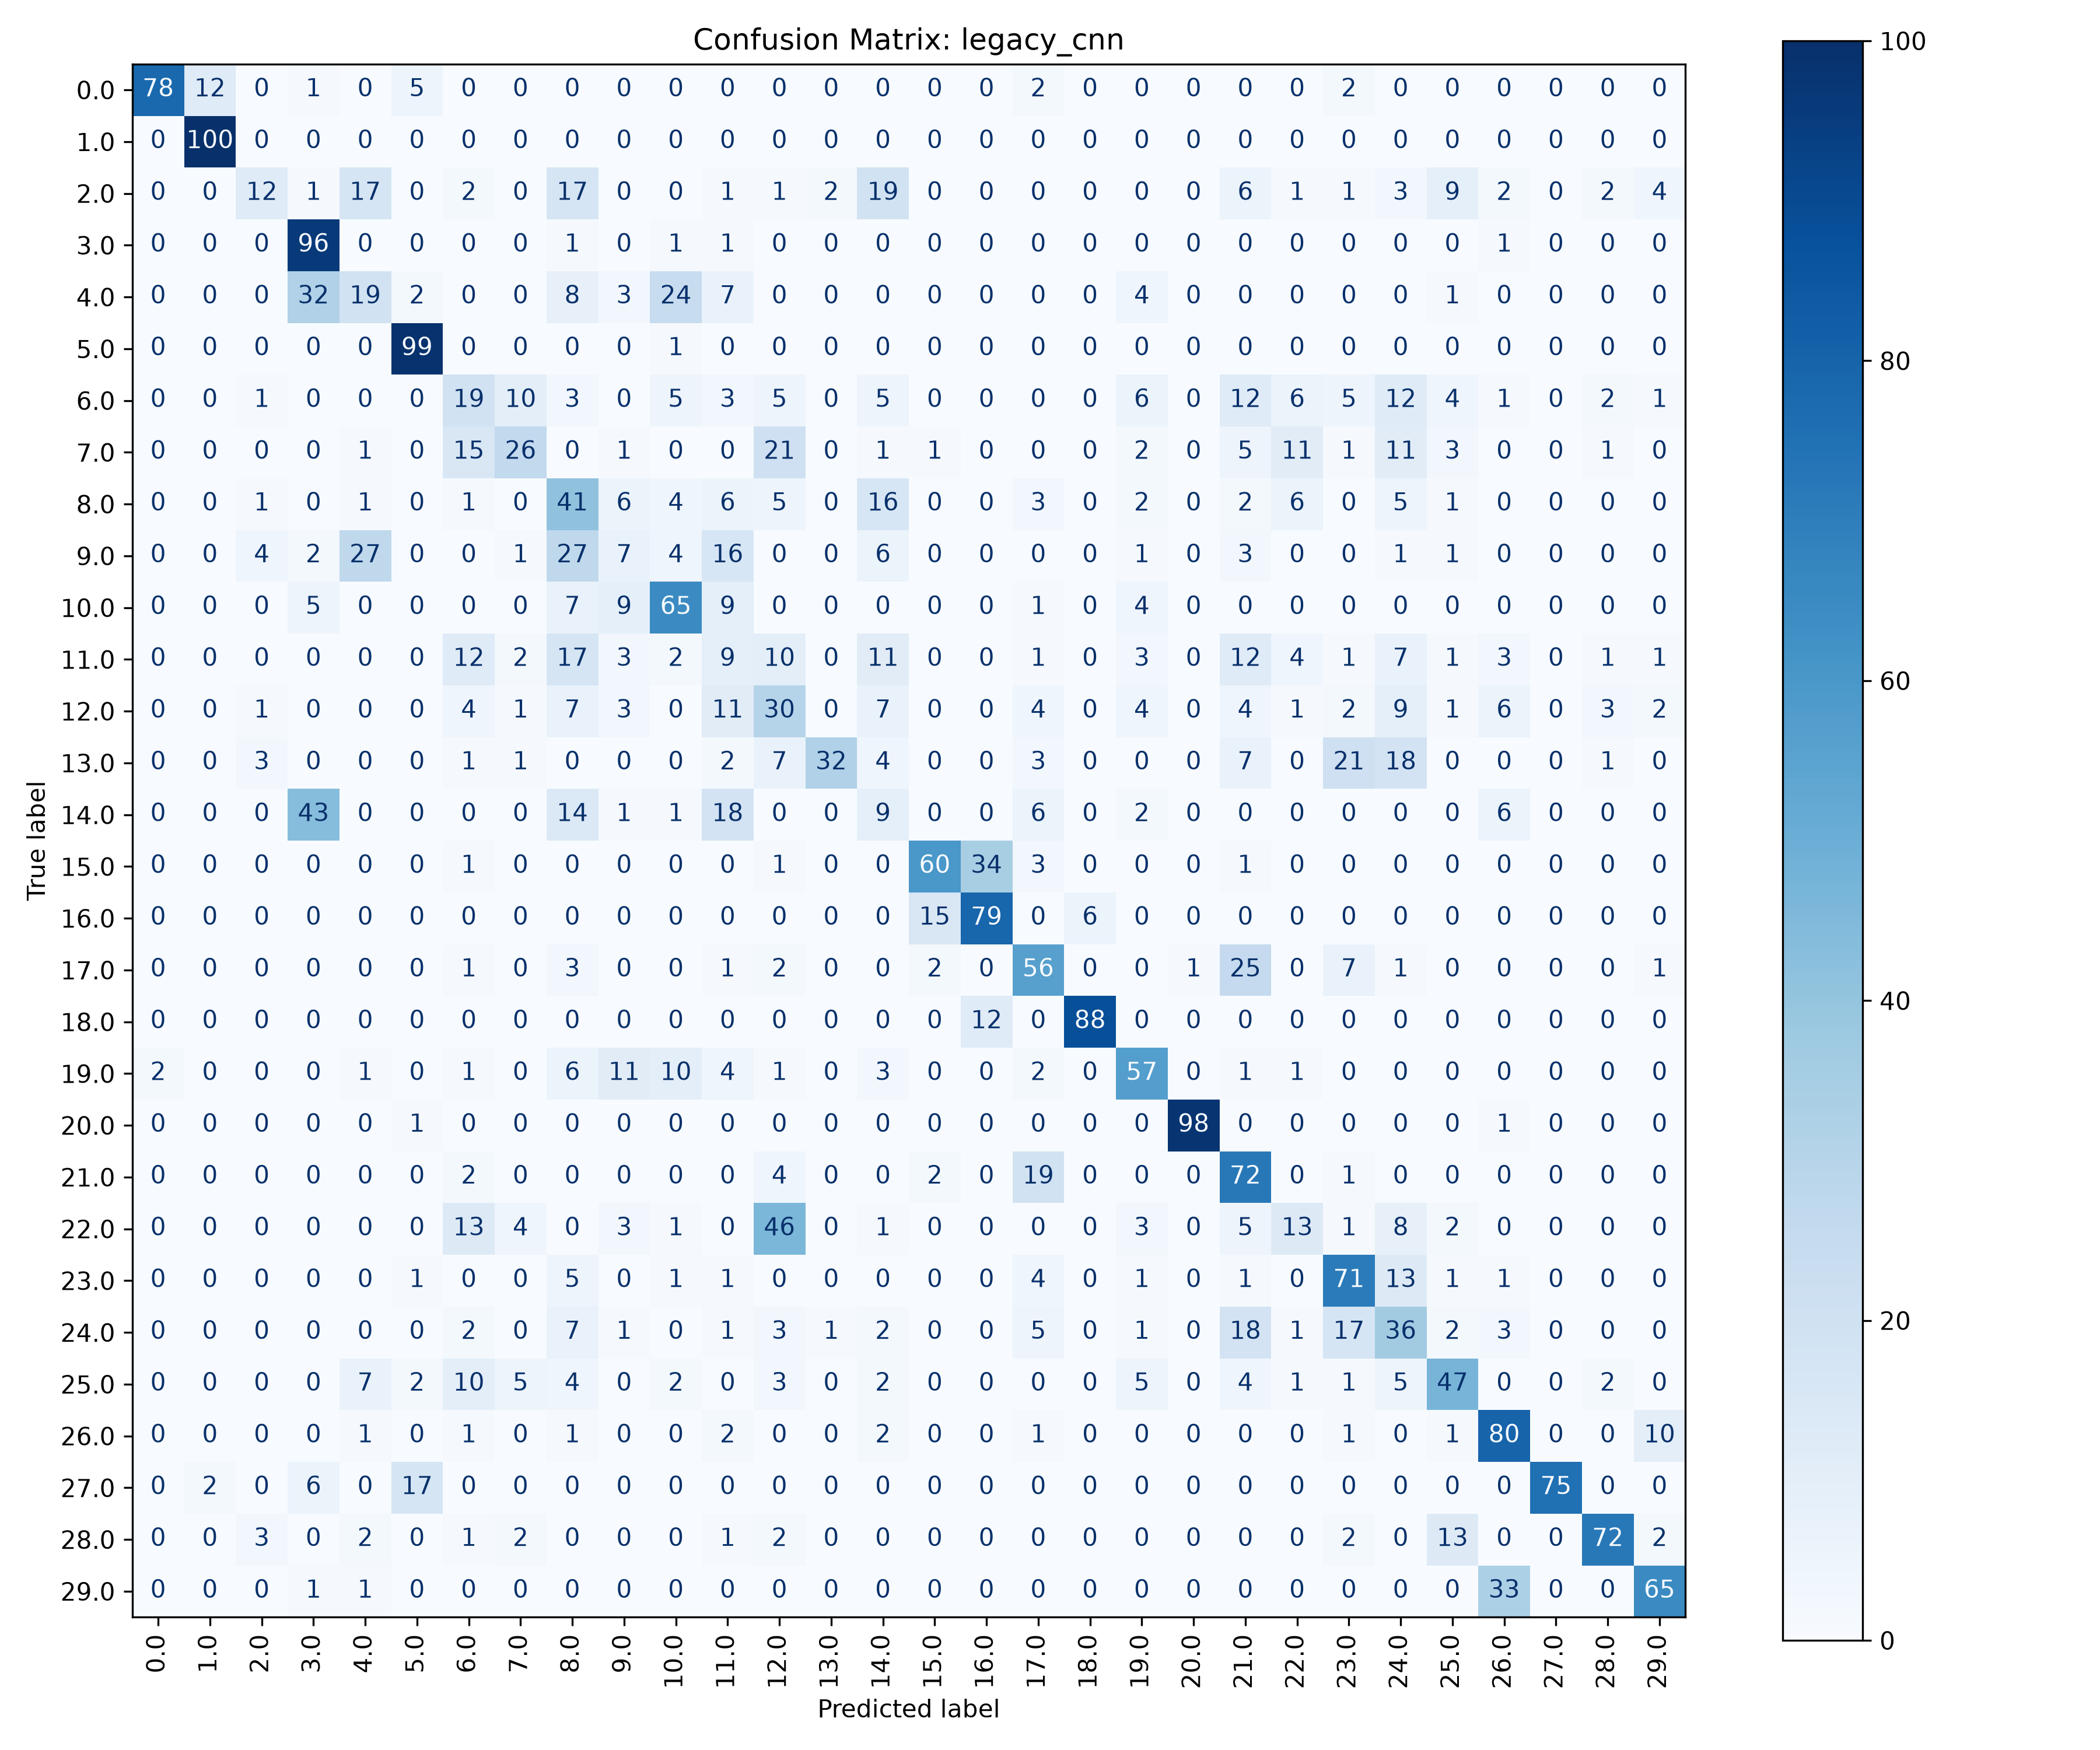
\includegraphics[width=0.48\textwidth]{confusion_matrix_legacy_cnn}}%
  \hfill
  \subfloat[1D ResNet\label{fig:cm-resnet}]{%
    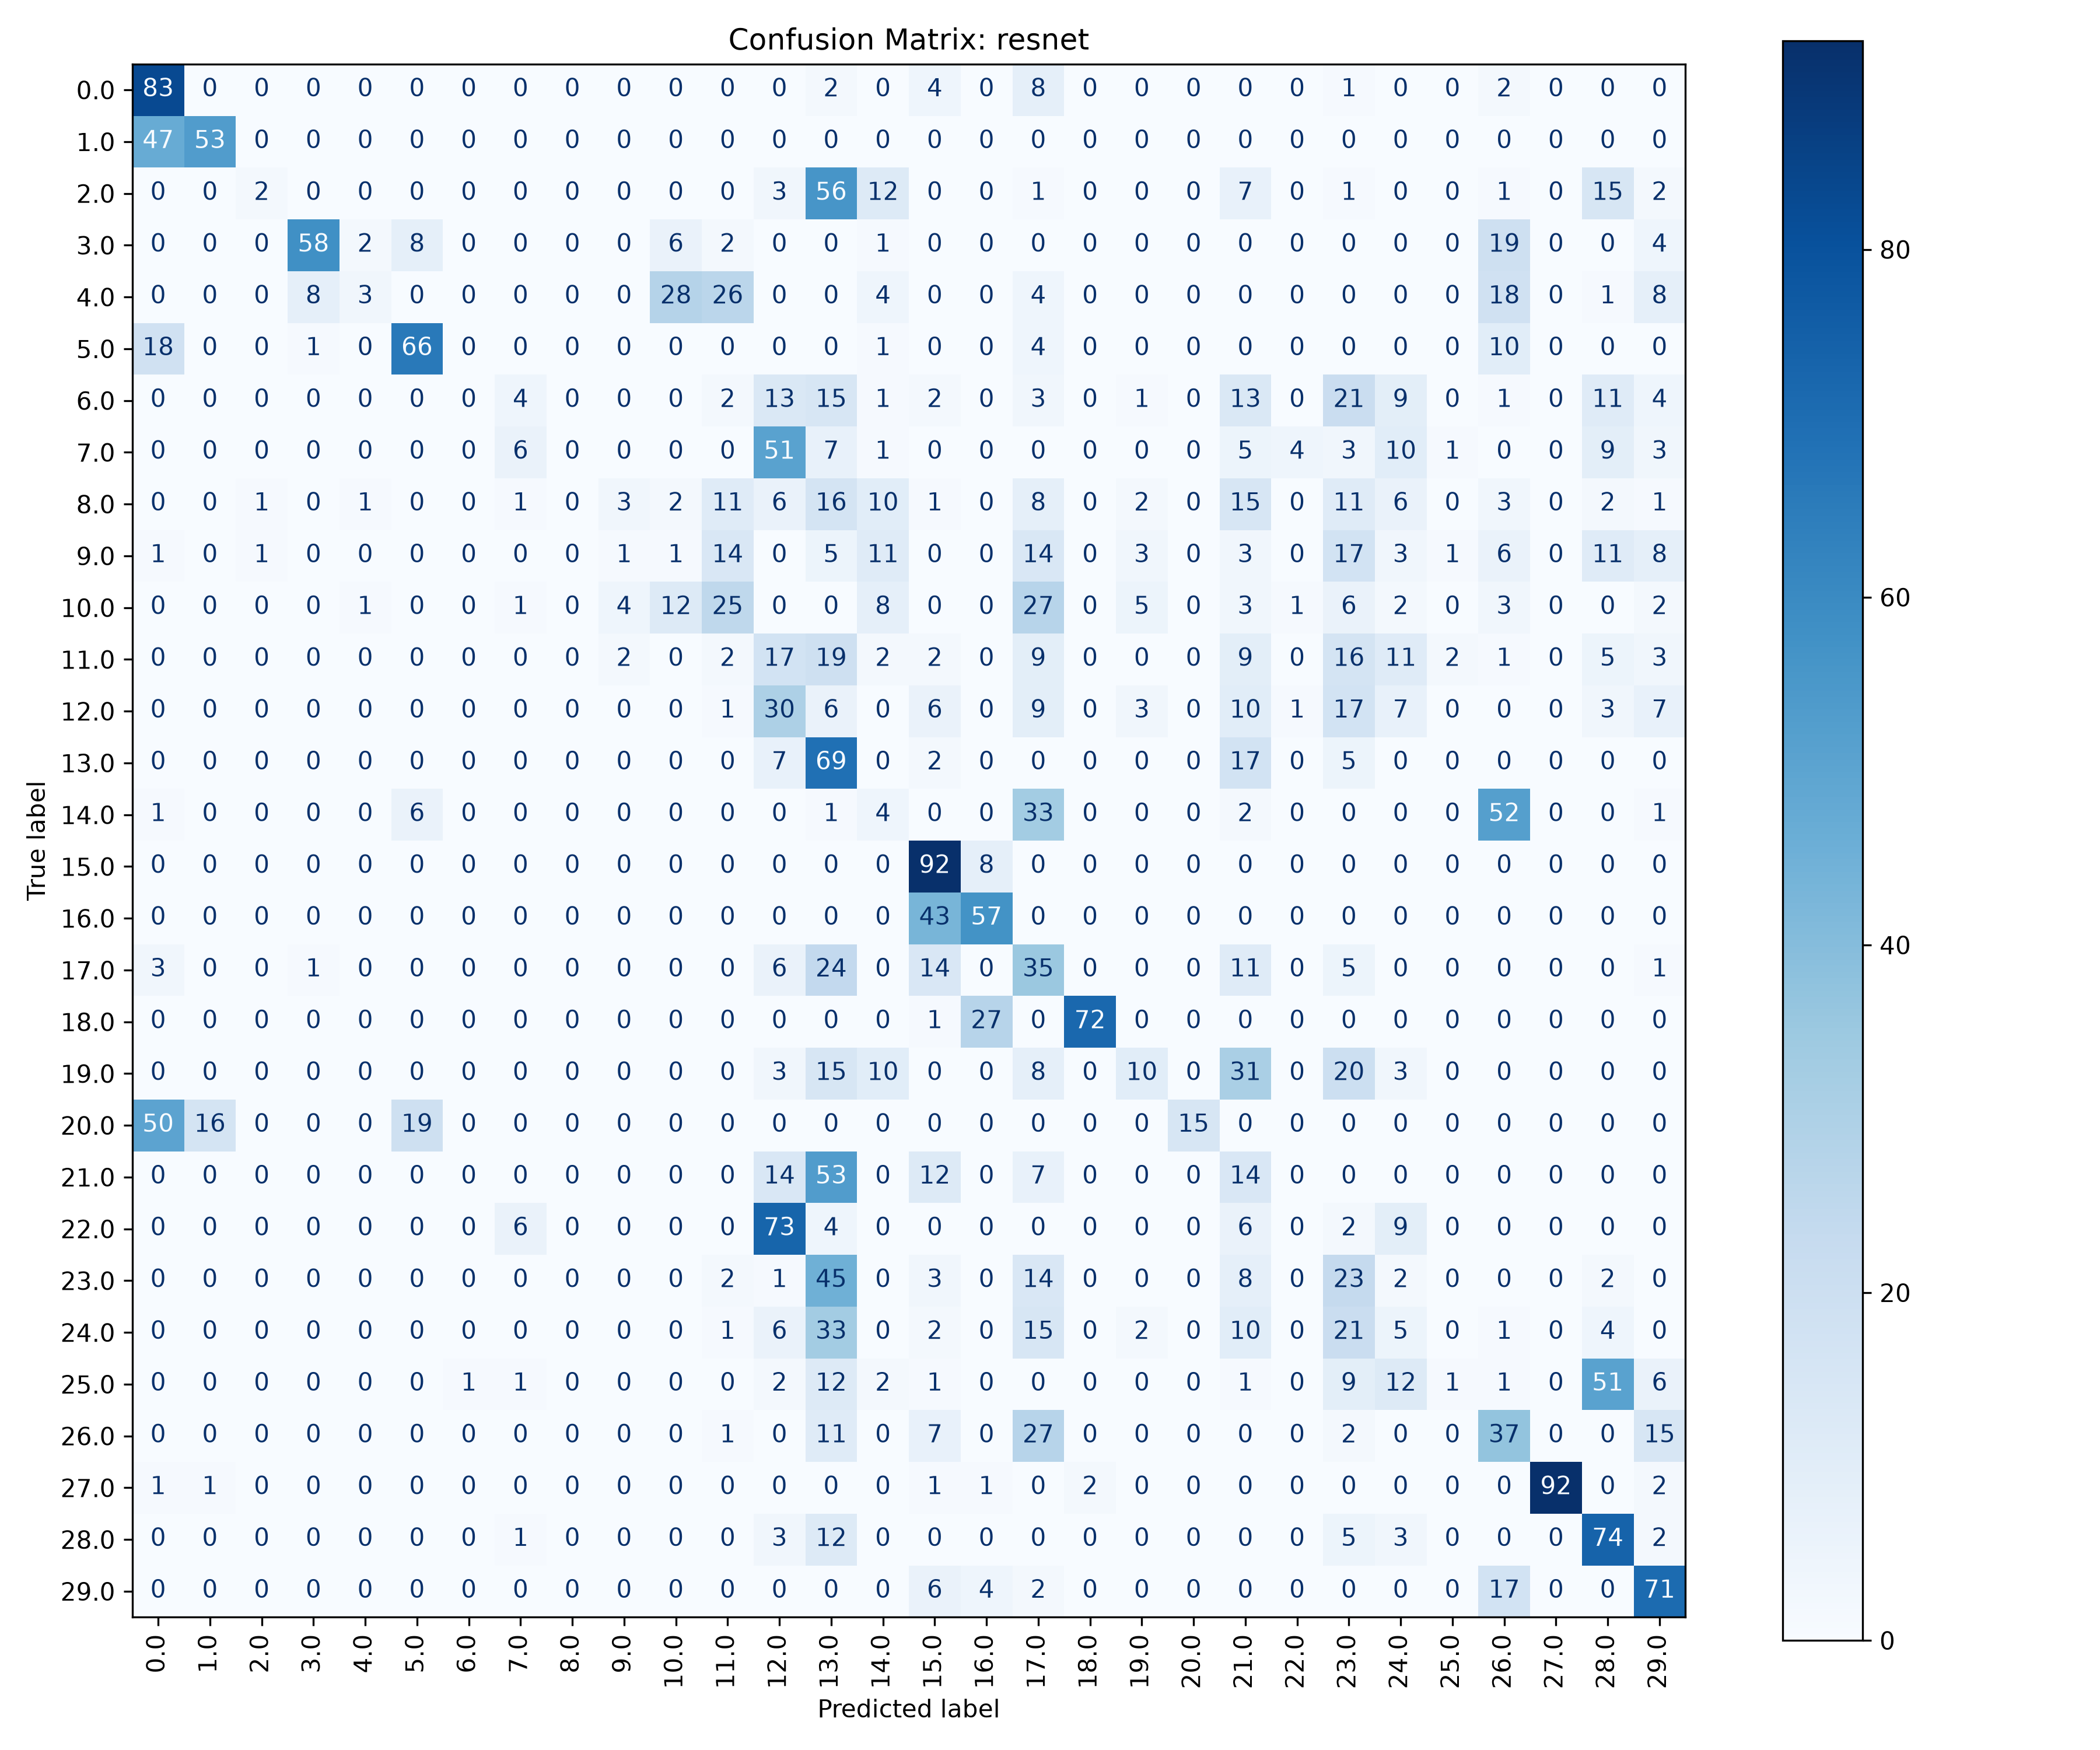
\includegraphics[width=0.48\textwidth]{confusion_matrix_resnet}}%
  \caption{Test-set confusion matrices for the 30-isolate task.
  \NOTE{These PNGs are placeholders from a 5-epoch run; regenerate them as
  vector PDFs from the final models.}}
  \label{fig:cm}
\end{figure*}

\Cref{fig:cm-plain,fig:cm-resnet} show that\dots
\NOTE{Discuss within-genus confusions, e.g.\ MSSA~3 vs.\ isogenic MRSA~1.}

\subsection{Empiric antibiotic treatment grouping}
Predictions over 30 isolates are mapped to the eight empiric-treatment
groups of \cite{ho2019rapid} (e.g.\ vancomycin for all \textit{Staphylococcus}
isolates; penicillin for streptococci and \textit{E.~faecalis}).
\NOTE{Also report patient-level accuracy on the clinical sets (majority
vote over 10 spectra), and state the patient-block assumption.}

\subsection{Binary drug resistance (MRSA vs.\ MSSA)}
A binary classifier is trained on the \textit{S.~aureus} isolates
(MRSA 1, 2 vs.\ MSSA 1, 2, 3). \Cref{fig:roc} shows ROC curves.

% ---- Example 4: placeholder until the figure exists ------------------
\begin{figure}[!t]
  \centering
  \figorplaceholder{fig_roc_mrsa.pdf}{4.5cm}
  \caption{ROC curves for MRSA vs.\ MSSA. The dashed diagonal is chance.}
  \label{fig:roc}
\end{figure}

\subsection{Robustness to noise and instrument drift}
\label{sec:res-noise}
\emph{Controlled SNR.} We add zero-mean Gaussian noise to test spectra so
that \eqref{eq:snr} reaches target values of \TBD{4, 3, 2, 1}. These are
simulated degradations, not new acquisitions. \emph{Instrument drift.}
We also report accuracy on the \sunit{2} test set before and after
fine-tuning, which measures transfer across a real change in optics
(\cref{fig:noise}).

% ---- Example 5: two sub-figures side by side inside ONE column -------
\begin{figure}[!t]
  \centering
  \subfloat[Accuracy vs.\ SNR\label{fig:noise-snr}]{%
    \figorplaceholder[0.48\figwidth]{fig_acc_vs_snr.pdf}{3cm}}%
  \hfill
  \subfloat[Fine-tuning gain\label{fig:noise-ft}]{%
    \figorplaceholder[0.48\figwidth]{fig_ft_gain.pdf}{3cm}}%
  \caption{Robustness. (a) Simulated SNR degradation. (b) Accuracy on the
  test set before and after fine-tuning.}
  \label{fig:noise}
\end{figure}

\subsection{Training dynamics and computational efficiency}
\Cref{fig:curves} shows loss curves and \cref{tab:cost} the cost of each
model. \NOTE{Add per-layer gradient-norm plots to support any
gradient-flow claim; report the epoch at which validation accuracy first
reaches 95\% of its maximum.}

% ---- Example 6: raster image (PNG) at column width -------------------
% Use PDF/EPS for plots whenever possible. A raster image must be at
% least 300 dpi at its printed size (3.5 in -> >= 1050 px wide).
\begin{figure}[!t]
  \centering
  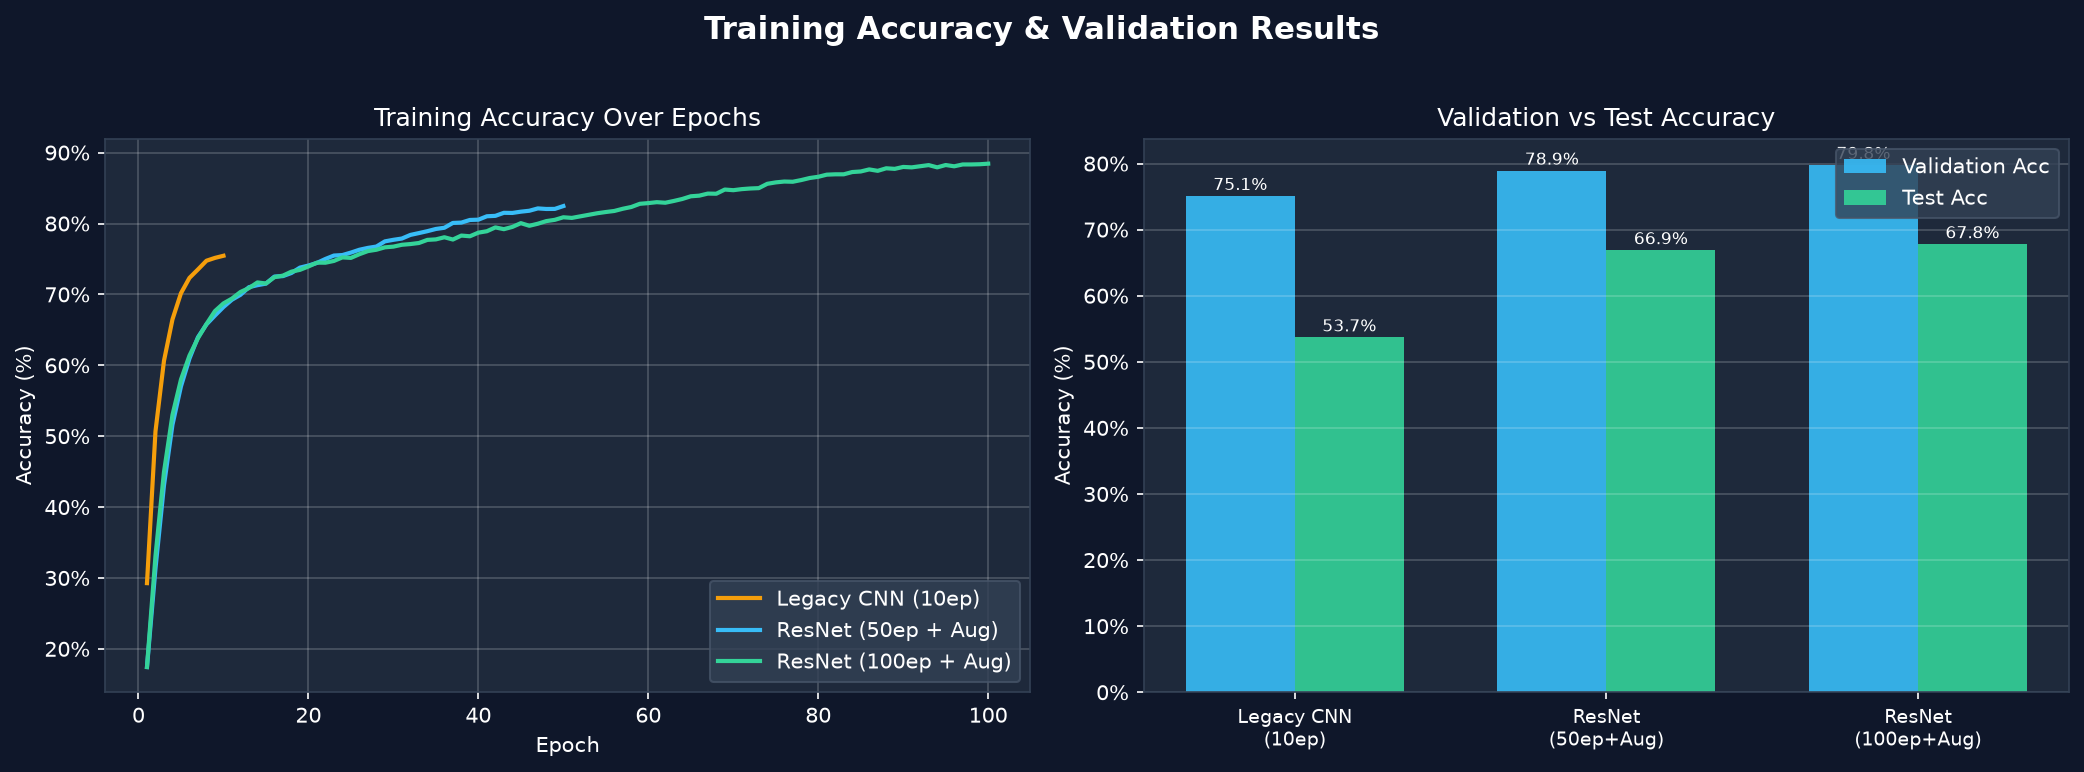
\includegraphics[width=\figwidth]{loss_curves}
  \caption{Training and validation loss. \NOTE{Placeholder image; replace
  with curves for the final configurations, mean $\pm$ s.d.\ bands.}}
  \label{fig:curves}
\end{figure}

\begin{table}[!t]
  \centering
  \caption{Model cost. Latency per spectrum, batch size 1.}
  \label{tab:cost}
  \begin{tabular}{@{}l r r r@{}}
    \toprule
    Model & Params (k) & CPU (ms) & GPU (ms) \\
    \midrule
    ResNet-25 & \TBD{} & \TBD{} & \TBD{} \\
    Plain-25  & \TBD{} & \TBD{} & \TBD{} \\
    \bottomrule
  \end{tabular}
\end{table}

%% =====================================================================
%% 7. DISCUSSION
%% =====================================================================
\section{Discussion}
\label{sec:discussion}

\subsection{Do skip connections matter for 1D spectra?}
\NOTE{Interpret the matched contrast: at 25 layers, does the plain twin
train worse (an optimisation problem \cite{glorot2010understanding},
visible in the gradient norms) or
generalise worse? Does the gap shrink at shallow depth?}

\subsection{Spectral feature retention}
\NOTE{Use saliency or Grad-CAM over wavenumber \cite{simonyan2014deep} to
show which peaks each model relies on, and whether strided convolutions
preserve peak positions better than pooling. Avoid comparisons to 2D
image features that no experiment supports.}

\subsection{Clinical and practical implications}
\NOTE{Accuracy vs.\ parameter count and latency for point-of-care
hardware; treatment-level accuracy is the clinically relevant number.}

\subsection{Limitations}
All results use one public dataset from one instrument; no new samples
were measured. SNR degradation is simulated. The release has no sample
identifiers, so variance between preparations cannot be separated from
variance within a preparation. \NOTE{Add: test-set reuse during earlier
exploratory work, if any.}

%% =====================================================================
%% 8. CONCLUSION
%% =====================================================================
\section{Conclusion}
\label{sec:conclusion}
\NOTE{3--5 sentences: the controlled finding, then concrete design
recommendations (depth, shortcuts, downsampling, kernel width) for 1D
spectroscopic classifiers.}

%% =====================================================================
%% Back matter expected by most journals
%% =====================================================================
\section*{Data and Code Availability}
The bacteria-ID dataset is available from the authors of
\cite{ho2019rapid}. Code, configuration files and per-run manifests are
available at \TBD{repository URL and commit hash}.

\section*{Author Contributions}
\TBD{CRediT statement, e.g.\ A.J.: conceptualisation, software,
investigation, writing -- original draft.}

\section*{Acknowledgment}
\TBD{Acknowledgments.}

\section*{Conflict of Interest}
The authors declare no competing interests.

\bibliographystyle{IEEEtran}
\bibliography{references}

%% =====================================================================
%% APPENDIX
%% =====================================================================
\appendices
\section{Pre-processing Ablation}
\label{app:preproc}
\NOTE{Table of test accuracy for full / no-ASPLS / no-despike / no-SavGol /
min--max only / none, 3 seeds each (results/ablation/).}

\end{document}
